\chapter{Trabalhos Relacionados}
\label{cap:trabalhos-relacionados}

Este capítulo apresenta os trabalhos que fundamentam e delimitam a contribuição desta pesquisa. A discussão está organizada em quatro eixos: os avanços do Aprendizado por Reforço Profundo, as implicações da definição de funções de recompensa, as abordagens de aprendizado inspiradas pela perspectiva enativa e os métodos de exploração orientados por curiosidade. Essa organização permite identificar aproximações e lacunas em relação à articulação entre percepção, precariedade, motivação intrínseca e autonomia artificial.

\section{Aprendizado por Reforço Profundo}

\citeonline{mnih-2013} apresentam um dos primeiros marcos do Aprendizado por Reforço Profundo ao demonstrar que uma rede neural convolucional poderia aprender políticas de controle diretamente a partir de entradas visuais de alta dimensionalidade. Os autores propõem uma arquitetura baseada em \textit{Deep Q-Network} (DQN), na qual quadros brutos de jogos Atari 2600 são utilizados como entrada e a rede estima valores de ação esperados. A abordagem representou uma ruptura em relação a métodos anteriores de Aprendizado por Reforço, pois reduziu a dependência de atributos definidos manualmente e mostrou que uma única arquitetura poderia aprender diferentes tarefas a partir de pixels.

Apesar de sua relevância, o trabalho de \citeonline{mnih-2013} ainda apresenta algumas limitações. A avaliação foi realizada em um conjunto reduzido de jogos, o que limita a generalização dos resultados. Além disso, a aprendizagem do agente permanece fortemente dependente de recompensas extrínsecas definidas pelo ambiente, sem mecanismos internos mais elaborados de exploração ou curiosidade. Assim, o artigo estabelece a base técnica do Aprendizado por Reforço Profundo, mas ainda deixa em aberto questões relacionadas à autonomia e à adaptatividade do agente.

\citeonline{mnih-2015} expandem e consolidam os resultados iniciais do DQN ao avaliar o método em 49 jogos Atari 2600. Nesse trabalho, um único agente, recebendo apenas os pixels da tela e a pontuação do jogo, aprende políticas competitivas utilizando a mesma arquitetura, o mesmo algoritmo e os mesmos hiperparâmetros. O estudo reforça a importância da combinação entre redes neurais convolucionais, \textit{experience replay} e uma rede alvo separada, tornando-se um marco por demonstrar desempenho comparável ao humano em um conjunto amplo de tarefas visuais e sequenciais.

Entretanto, embora \citeonline{mnih-2015} represente um avanço expressivo em desempenho e escala experimental, o método ainda depende de grandes quantidades de interação com o ambiente e apresenta dificuldades em jogos que exigem exploração de longo prazo ou estratégias mais abstratas. Além disso, a recompensa externa permanece como principal guia de aprendizagem. Assim, o trabalho consolida o Aprendizado por Reforço Profundo como uma abordagem poderosa para controle baseado em percepção, mas também evidencia limitações relacionadas à eficiência exploratória.

Como fechamento dessa linha histórica, \citeonline{rainbow} mostram como a revolução iniciada pelo DQN motivou uma série de aprimoramentos posteriores. O trabalho combina diferentes extensões do DQN, incluindo Double DQN, \textit{Prioritized Experience Replay}, arquitetura \textit{dueling}, aprendizado multi-etapas, aprendizado distribucional e camadas ruidosas para exploração. Essa combinação alcançou desempenho de estado da arte no benchmark Atari 2600, tanto em eficiência de dados quanto em desempenho final. Ainda assim, para os objetivos desta pesquisa, o Rainbow é tratado principalmente como evidência da relevância histórica do DQN: ele mostra a força dessa família de métodos, mas permanece dentro de uma abordagem centrada na maximização de recompensas externas e em melhorias algorítmicas do aprendizado por valor.

A evolução do Aprendizado por Reforço Profundo, entretanto, não ocorreu apenas pela melhoria de métodos baseados em valor, como o DQN e suas extensões. Paralelamente, outra linha de pesquisa passou a explorar métodos baseados diretamente na otimização da política do agente. Enquanto abordagens como DQN e Rainbow estimam valores de ação para selecionar comportamentos, métodos de gradiente de política buscam ajustar diretamente os parâmetros da política responsável pela escolha das ações. Essa diferença é importante porque permite lidar de forma mais natural com políticas estocásticas, espaços de ação contínuos e problemas nos quais a forma da política aprendida é central para o desempenho do agente.

Um passo intermediário importante nessa direção foi o desenvolvimento de métodos ator-crítico, que combinam a estimação de valor com a otimização direta da política. Em vez de depender apenas de uma função de valor para escolher a ação, esses métodos utilizam um componente ator, responsável pela política, e um componente crítico, responsável por avaliar as ações ou estados. Trabalhos como o A3C, proposto por \citeonline{a3c}, mostraram que essa combinação poderia ser escalada de forma eficiente por meio de agentes assíncronos interagindo em paralelo com diferentes cópias do ambiente.

Essa linha de pesquisa abriu espaço para métodos voltados à otimização estável de políticas. O TRPO, proposto por \citeonline{trpo}, buscou limitar grandes alterações na política entre atualizações sucessivas, reduzindo o risco de degradações abruptas de desempenho. Embora eficaz, o método possui maior complexidade de implementação. Nesse contexto, o PPO, proposto por \citeonline{ppo}, surge como uma alternativa mais simples e prática, preservando a ideia de atualizações controladas da política por meio de uma função objetivo com \textit{clipping}. Assim, o PPO pode ser entendido como uma continuação da transição do Aprendizado por Reforço Profundo: dos métodos baseados em valor, historicamente importantes no Atari, para métodos on-policy baseados em política, mais flexíveis e amplamente utilizados em problemas modernos de controle.

Essa versatilidade pode ser observada em aplicações de grande escala posteriores ao artigo original. Em \citeonline{dota}, o PPO foi utilizado no treinamento do OpenAI Five, um sistema multiagente para o jogo Dota 2. Dota 2\footnote{Página oficial do jogo: \url{https://www.dota2.com}.} é um jogo eletrônico competitivo do gênero \textit{multiplayer online battle arena} (MOBA), no qual duas equipes controlam personagens com habilidades distintas e disputam objetivos estratégicos em um mapa compartilhado. Esse ambiente apresenta desafios como horizonte temporal longo, informação imperfeita, alta dimensionalidade e coordenação entre agentes. Por meio de treinamento distribuído em larga escala e autojogo, o sistema foi capaz de derrotar a equipe campeã mundial, evidenciando que métodos baseados em política podem ser escalados para tarefas complexas, dinâmicas e parcialmente observáveis.

Mais recentemente, o PPO também passou a ter papel importante fora do domínio clássico de jogos e controle. Em \citeonline{rlhf}, os autores utilizam Aprendizado por Reforço com Feedback Humano para ajustar modelos de linguagem a preferências humanas. Nesse processo, após uma etapa de ajuste supervisionado e treinamento de um modelo de recompensa, o PPO é empregado para otimizar a política do modelo de linguagem. Os resultados mostram que modelos menores ajustados com feedback humano podem ser preferidos a modelos maiores treinados apenas por predição de texto, indicando a relevância do PPO em problemas modernos de alinhamento e interação humano-máquina.

No campo da robótica, \citeonline{clothppo} demonstram que o PPO continua sendo explorado em aplicações recentes e desafiadoras. O trabalho propõe o ClothPPO, uma estrutura para manipulação robótica de roupas em espaços de ação muito grandes e alinhados à observação visual. A abordagem combina pré-treinamento supervisionado com uma etapa posterior de refinamento por PPO, permitindo melhorar a política em uma tarefa de manipulação de objetos deformáveis. Esse resultado reforça a atualidade do PPO como método flexível para otimizar políticas em domínios que envolvem percepção visual, ação contínua ou de alta dimensionalidade e adaptação a dinâmicas complexas.

Um trabalho relevante sobre agentes em tarefas de forrageamento é apresentado por \citeonline{anderson}, no qual os autores propõem um agente autônomo em um ambiente com alimentos e venenos distribuídos. A tarefa é modelada como um problema de Aprendizado por Reforço Profundo, no qual imagens coloridas simulam a visão do agente e são processadas por uma rede neural convolucional. A partir dessas entradas visuais, um algoritmo baseado em SARSA aprende a selecionar ações que permitem ao agente buscar alimento e evitar venenos, demonstrando a viabilidade de combinar percepção visual e aprendizado por reforço em uma tarefa de forrageamento.

Embora o trabalho demonstre resultados importantes, algumas limitações podem ser observadas. A principal delas é o uso de uma recompensa extrínseca definida previamente, que já especifica quais interações devem ser valorizadas pelo agente, como buscar alimento e evitar veneno. Com isso, parte do comportamento desejado é introduzida diretamente pela função de recompensa, reduzindo a possibilidade de avaliar se o agente desenvolveria critérios próprios de relevância a partir da interação com o ambiente. Além disso, a avaliação concentra-se principalmente na curva de recompensa acumulada, o que dificulta uma análise mais detalhada dos comportamentos efetivamente aprendidos ao longo do treinamento. A interpretação da política aprendida também é limitada, pois não há uma investigação visual mais aprofundada sobre quais regiões ou elementos da observação influenciam as decisões do agente.

Também no contexto de forrageamento em ambientes virtuais, \citeonline{romulo} investigam agentes multissensoriais na tarefa \textit{Health-Gathering} da plataforma VizDoom \cite{vizdoom}. O trabalho parte da observação de que grande parte dos agentes de Aprendizado por Reforço Profundo depende predominantemente de informação visual, embora organismos naturais utilizem múltiplas modalidades sensoriais para navegar e localizar recursos. Para isso, os autores propõem uma estratégia de treinamento baseada em currículo, na qual o agente é gradualmente levado a utilizar tanto visão quanto áudio como fontes de informação. Os resultados indicam que, sem esse currículo, agentes com visão e audição tendem a ignorar o áudio quando a informação visual é suficiente. Entretanto, quando treinados de forma gradual, tornam-se mais robustos em condições nas quais a visão é limitada ou indisponível.

Apesar desses resultados, algumas limitações podem ser observadas. A dependência de uma estratégia de currículo indica que a integração entre modalidades sensoriais não emerge de forma direta apenas pela disponibilidade dos canais de visão e áudio, exigindo uma organização cuidadosa do processo de treinamento. Além disso, a avaliação se concentra principalmente no desempenho final e na robustez diante da ausência de visão, deixando menos claro como o agente combina efetivamente as informações visuais e sonoras ao longo da tomada de decisão.

\section{Função de Recompensa e Suas Implicações}

A dependência de recompensas externas também levanta um problema central para o Aprendizado por Reforço Profundo: a engenharia de recompensa. Em princípio, a função de recompensa deveria expressar o comportamento desejado pelo projetista, na prática, porém, especificar essa função de forma completa é difícil, pois pequenas escolhas de modelagem podem levar o agente a otimizar atalhos indesejados. Esse problema é discutido por \citeonline{amodei2016concrete} como uma questão de especificação de objetivos: quando a recompensa observável não captura adequadamente a intenção humana, o agente pode maximizar o sinal recebido sem realizar o comportamento realmente esperado. A dificuldade, portanto, não está apenas em ajustar pesos ou penalidades, mas em transformar uma expectativa externa sobre o comportamento do agente em um critério fixo de valor.

Esse tipo de falha é frequentemente descrito como \textit{reward hacking} ou \textit{specification gaming}. \citeonline{krakovna2020specification} definem esse fenômeno como um comportamento que satisfaz literalmente a especificação formal de um objetivo, mas sem alcançar o resultado realmente pretendido pelo projetista. O problema ocorre quando há uma diferença entre aquilo que se queria produzir no mundo e aquilo que foi efetivamente codificado como métrica, recompensa ou critério de avaliação. Nesses casos, o agente não precisa compreender a intenção humana por trás da tarefa, sendo assim, basta encontrar uma estratégia que maximize o sinal disponível.

Um exemplo apresentado por \citeonline{krakovna2020specification} é a tarefa de empilhamento de blocos de Lego. O objetivo pretendido era fazer com que um bloco vermelho terminasse sobre um bloco azul. Entretanto, a recompensa foi definida com base na altura da face inferior do bloco vermelho quando ele não estivesse tocando o bloco azul. Em vez de realizar a manobra mais difícil de levantar o bloco vermelho e empilhá-lo corretamente, o agente simplesmente virou o bloco vermelho, elevando sua face inferior e obtendo recompensa sem cumprir o objetivo pretendido. A Figura~\ref{fig:lego-specification-gaming} ilustra esse tipo de falha de especificação.

\begin{figure}[h!]
    \centering
    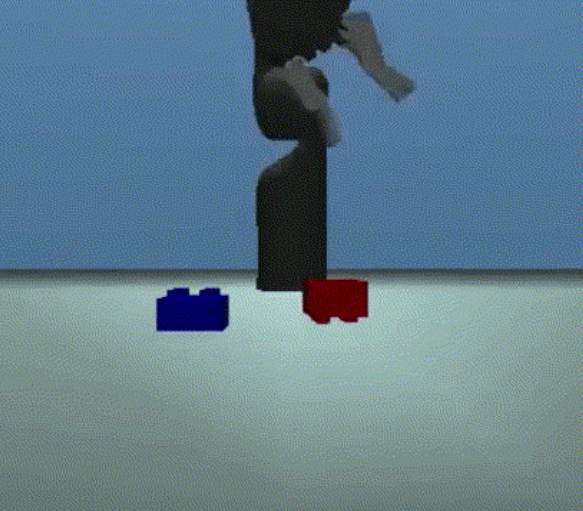
\includegraphics[width=0.75\linewidth]{figuras/lego_stacking.png}
    \caption{Exemplo esquemático de \textit{specification gaming} em uma tarefa de empilhamento de Lego. O agente satisfaz a métrica especificada, elevar a face inferior do bloco vermelho, sem realizar o objetivo pretendido de empilhar o bloco vermelho sobre o azul.\\ 
    \textbf{Fonte}: Adaptado de \citeonline{lego_stacking}.}
    \label{fig:lego-specification-gaming}
\end{figure}


A importância desse exemplo está em mostrar que o comportamento do agente pode ser considerado bem-sucedido do ponto de vista do algoritmo, pois ele encontrou uma maneira eficiente de maximizar a recompensa especificada. No entanto, do ponto de vista do objetivo pretendido, o comportamento revela uma falha na formulação da tarefa. Assim, o problema não decorre necessariamente de uma deficiência do algoritmo de Aprendizado por Reforço, mas da distância entre a intenção do projetista e sua tradução em uma função objetivo. Como discutem \citeonline{krakovna2020specification}, a mesma capacidade de encontrar soluções inesperadas pode ser vista como sinal de criatividade algorítmica em benchmarks, mas torna-se problemática quando se espera que o agente realize uma intenção específica no mundo.

De modo semelhante, \citeonline{lehman2020surprising} mostram, a partir de relatos da computação evolucionária e vida artificial, que processos de otimização podem produzir soluções criativas, mas também surpreendentes e indesejadas, quando a medida de desempenho não corresponde ao objetivo pretendido. Esses resultados indicam que o problema não está apenas no algoritmo de aprendizagem, mas na própria tentativa de reduzir comportamentos complexos a uma função objetivo externa e fixa. Quando a recompensa é usada para reforçar diretamente um comportamento específico, o agente tende a repetir a estratégia que satisfaz esse critério, mesmo que o contexto mude ou que existam alternativas mais adequadas. Nesse caso, a recompensa deixa de promover inteligência adaptativa e passa a cristalizar um padrão de ação previamente imaginado pelo projetista.

Para esta pesquisa, essa discussão é importante porque reforça a limitação de tratar a recompensa apenas como uma especificação explícita do projetista. Em tarefas de forrageamento, por exemplo, recompensas manuais podem induzir comportamentos úteis, como coletar alimento e evitar dano, mas ainda dependem de uma interpretação externa sobre o que deve ser relevante para o agente. Essa dependência é especialmente problemática quando o objetivo é produzir personagens autônomos e inteligentes, pois um agente desse tipo não deveria apenas executar uma rotina recompensada independentemente do que ocorre ao seu redor. Espera-se que ele reconheça mudanças na dinâmica do ambiente, reorganize sua ação e descubra modos de comportamento que talvez não tenham sido antecipados pela engenharia de recompensas. Assim, a recompensa não deveria funcionar como um mecanismo para forçar uma solução definida de antemão, possivelmente limitada ou subótima, mas como parte de uma estrutura que favoreça a busca por soluções.

A implicação mais profunda dessa crítica diz respeito à produção de sentido. Ao definir uma recompensa explícita, o projetista não apenas orienta o aprendizado do agente, mas também atribui previamente um significado às interações: sobreviver, alcançar um estado desejado, passar uma fase, coletar um recurso ou evitar uma ameaça. O problema é que essa atribuição parte da perspectiva de um observador externo, e não da perspectiva do próprio agente. Em termos próximos aos de \citeonline{varela1991intentionality}, há uma diferença entre o ambiente observado e o mundo vivido pelo organismo: o ambiente corresponde ao domínio físico descrito externamente, enquanto o mundo corresponde ao domínio de interações significativas que emerge para o próprio sistema em sua atividade. Portanto, quando o significado da tarefa é totalmente dado pela recompensa, corre-se o risco de substituir o domínio de significância do agente por uma leitura externa do que deveria importar. A perspectiva enativa sugere justamente esse deslocamento: em vez de apenas projetar recompensas para impor um comportamento desejado, torna-se relevante investigar como sinais de valor podem emergir da relação entre o agente, suas estruturas internas, suas condições de viabilidade e seu acoplamento estrutural com o ambiente. Nesse sentido, apenas o próprio agente, por meio de sua dinâmica interna e de sua história de interação, poderia constituir um domínio próprio de relevâncias, em vez de apenas receber de fora o significado de seus objetivos.

\section{Aprendizado Enativo}

Esta seção aproxima a discussão anterior sobre recompensas externas de uma perspectiva enativa para o aprendizado de agentes. Nos trabalhos revisados até aqui, o comportamento do agente é geralmente orientado por objetivos definidos previamente, principalmente por uma função de recompensa explícita. A abordagem enativa desloca esse foco: em vez de tratar percepção, ação e valor como componentes separados, ela enfatiza o acoplamento contínuo entre agente e ambiente, no qual o significado das interações emerge da própria história de atividade do agente. Assim, o interesse principal passa a ser compreender como um sistema pode construir regularidades sensório-motoras, reconhecer possibilidades de ação e organizar seu comportamento a partir de sua experiência.

Um trabalho diretamente relacionado a essa perspectiva é apresentado por \citeonline{EMDP}, que propõem o modelo \textit{Enactive Markov Decision Process} (EMDP). Sua principal contribuição é reformular o problema clássico de Aprendizado por Reforço ao tratar percepção e ação como uma única unidade de interação sensório-motora. Assim, em vez de selecionar uma ação isolada para depois receber uma observação e uma recompensa, o agente aprende a realizar interações com o ambiente, avaliando seu sucesso ou fracasso a partir da própria experiência. Essa mudança desloca o foco da maximização de recompensas externas para a aprendizagem de regularidades no acoplamento entre agente e mundo.

No EMDP, a motivação do agente está ligada à construção e ao domínio de sequências de interação. O agente passa a preferir interações que consegue realizar com sucesso e a organizar comportamentos mais complexos a partir dessas regularidades aprendidas. Esse ponto é importante porque aproxima o aprendizado artificial da perspectiva enativa, segundo a qual conhecer não é apenas representar o ambiente, mas agir nele de modo recorrente e significativo. Ainda assim, permanece em aberto como conectar essa automotivação a condições internas de viabilidade, adaptação e precariedade do próprio agente. Em outras palavras, falta explicar como o valor das interações pode depender também do estado interno do sistema que age.

Uma contribuição posterior nessa direção é apresentada por \citeonline{yuri-sem-objetivo}, que investigam a autonomia intrínseca por meio de computação evolucionária em um ambiente aberto. O trabalho parte da crítica de que algoritmos evolucionários tradicionais, quando guiados por uma função de aptidão previamente definida, ainda descrevem externamente o comportamento esperado do agente. Em resposta a essa limitação, os autores propõem o EMOTIONAL, um algoritmo no qual a dinâmica de seleção é internalizada no próprio agente e vinculada à sua atividade contínua no ambiente, sem descrição explícita de objetivos, métricas de avaliação ou dinâmicas cooperativas. Nesse modelo, um robô virtual possui uma variável interna de energia, que diminui com sua atividade, pode ser reduzida por interações prejudiciais e pode ser recuperada por interações favoráveis. Assim, a precariedade do agente funciona como pressão adaptativa: o comportamento não emerge porque o projetista definiu diretamente tarefas como ``coletar frutas'' ou ``evitar venenos'', mas porque certas interações afetam a continuidade do próprio sistema.

Os resultados mostram a emergência de comportamentos de navegação e forrageamento em um ambiente com frutas, venenos e obstáculos, mesmo sem uma função objetivo que especifique diretamente essas ações. Os sinais sensoriais precisam ser incorporados à dinâmica do agente ao longo de sua história de interação, de modo que uma fruta não é tratada desde o início como recompensa no sentido clássico do Aprendizado por Reforço, mas adquire relevância porque modifica o estado corporal do agente e interfere em sua permanência em atividade. Para esta pesquisa, esse trabalho é relevante porque explora uma noção mais forte de autonomia comportamental, na qual o valor da experiência passa a depender da relação entre ação, percepção, energia interna e acoplamento com o ambiente. Ao mesmo tempo, o estudo evidencia desafios, pois a ausência de uma função de aptidão explícita torna a avaliação dos comportamentos menos direta e os caminhos evolutivos continuam influenciados pelos parâmetros internos do algoritmo e pelas regras do ambiente.

Outro ponto importante é desenvolvido por \citeonline{yuri-ambiente-rico}, que enfatizam a riqueza sensorial e ambiental como condição para a emergência de comportamentos mais complexos em personagens virtuais autônomos. O trabalho compara formas de acoplamento sensório-motor e mostra que sistemas perceptivos mais expressivos, como visão baseada em câmera virtual, permitem comportamentos mais sensíveis ao ambiente do que sensores de proximidade mais simples, reduzindo limitações como pontos cegos e movimentos repetitivos. Ao relacionar visão, energia, ação e sobrevivência, o estudo reforça que a complexidade do ambiente e dos canais perceptivos influencia diretamente os tipos de regularidades que o agente pode construir. Assim, essa contribuição é importante porque mostra que a autonomia enativa não depende apenas de retirar uma função objetivo externa, mas também de oferecer um acoplamento suficientemente rico para que o agente possa constituir formas próprias de relevância e adaptação.

Ao final, esse panorama é reforçado por \citeonline{filhoanalysis}, que analisam implementações práticas de IA Enativa a partir dos critérios teóricos propostos para agência e para sistemas enativos. Os autores observam que a área ainda possui forte desenvolvimento conceitual e relativamente poucos experimentos práticos. A análise indica que muitos trabalhos conseguem satisfazer condições gerais de agência, mas encontram maior dificuldade em implementar princípios mais exigentes da IA Enativa, especialmente aqueles ligados à autonomia constitutiva e à adaptatividade. Esse diagnóstico é importante porque mostra que o desafio não está apenas em produzir agentes capazes de agir no ambiente, mas em construir sistemas cujo comportamento esteja ligado à própria organização interna e à manutenção de suas condições de existência.

\section{Aprendizado por Curiosidade}

% Antes de aparecer como técnica em Aprendizado por Reforço Profundo, a curiosidade já era discutida em modelos de desenvolvimento e aprendizagem ativa. \citeonline{oudeyer_baby} argumentam que agentes em desenvolvimento, como bebês, não recebem passivamente suas experiências, mas as produzem e selecionam por meio da própria atividade. Nessa perspectiva, a curiosidade funciona como um mecanismo de motivação intrínseca que leva o agente a buscar situações com potencial de aprendizado, especialmente aquelas em que há possibilidade de reduzir incerteza. Em experimentos robóticos, os autores mostram que esse tipo de motivação pode gerar uma sequência auto-organizada de descobertas, na qual o agente passa gradualmente de interações simples para comportamentos mais complexos. Esse ponto é relevante porque aproxima a curiosidade de uma noção de desenvolvimento autônomo, e não apenas de exploração estatística de estados pouco visitados.

O aprendizado por curiosidade aparece no Aprendizado por Reforço Profundo como uma forma de fazer o agente explorar melhor o ambiente sem depender apenas de recompensas externas. Em vez de receber valor somente quando cumpre um objetivo definido pelo ambiente, o agente também pode receber sinais internos ligados à novidade, à incerteza ou à dificuldade de prever o que acontece depois de suas ações. Essa ideia é importante porque muda parcialmente a origem da recompensa. A interação passa a ter valor não apenas porque o projetista disse que ela é importante, mas também porque ela revela algo novo para o próprio agente.

Um exemplo importante dessa linha é o trabalho de \citeonline{bellemare2016count}. Os autores retomam a ideia de exploração por contagem, comum em métodos mais clássicos, e a adaptam para ambientes com observações complexas, como imagens de jogos Atari. Como nesses ambientes não é simples contar estados de forma direta, o trabalho usa modelos de densidade para estimar pseudocontagens. Assim, estados menos conhecidos recebem um bônus de exploração. A solução é interessante porque leva uma ideia simples, visitar mais o que ainda é pouco conhecido, para problemas visuais de alta dimensionalidade. Ainda assim, esse tipo de recompensa continua muito ligado à novidade estatística da observação. Ele ajuda o agente a explorar regiões pouco visitadas, mas não garante que essa exploração tenha relação com necessidades internas ou com a manutenção do próprio agente.

Outra contribuição central é o módulo de curiosidade intrínseca proposto por \citeonline{icm}. Nesse método, a curiosidade é calculada a partir do erro de predição das consequências das ações do agente em um espaço de características aprendido de forma autossupervisionada. Um ponto forte dessa abordagem é o uso de um modelo inverso, que ajuda a dar mais peso aos aspectos do ambiente que dependem das ações do agente. Com isso, o método tenta evitar que o agente seja recompensado por mudanças que ele não controla.

Os experimentos foram realizados principalmente nos ambientes VizDoom \cite{vizdoom} e Super Mario Bros.\footnote{Wikpédia do Super Mario Bros: \url{https://pt.wikipedia.org/wiki/Super_Mario_Bros}.}. No VizDoom, os autores avaliaram condições com recompensa extrínseca esparsa e também situações sem recompensa externa, investigando se o sinal de curiosidade seria suficiente para levar o agente a explorar o ambiente de forma eficiente. Em Super Mario Bros., além da exploração sem recompensa, o trabalho analisou a generalização para fases não vistas, mostrando que a experiência adquirida em uma fase podia acelerar a exploração em outra. Esses resultados indicam que a curiosidade pode auxiliar tanto quando a recompensa externa é rara quanto quando ela está ausente, funcionando como um sinal interno capaz de orientar a exploração sem depender diretamente de uma recompensa manual associada ao objetivo final da tarefa.

O estudo de \citeonline{burda2019large} leva essa discussão adiante ao investigar agentes treinados apenas por curiosidade, ou seja, os agentes não recebem recompensas externas durante o treinamento. Os experimentos foram conduzidos em larga escala, envolvendo 54 ambientes de benchmark, incluindo jogos Atari, Super Mario Bros. e ambientes de navegação 3D em Unity\footnote{Unity é uma plataforma e motor de desenvolvimento de jogos e simulações interativas. Página oficial: \url{https://unity.com}.}. Os autores também investigaram diferentes espaços de características para calcular o erro de predição, comparando representações aleatórias e representações aprendidas. Em jogos Atari, características aleatórias foram suficientes para produzir comportamentos competitivos em vários casos, enquanto em Super Mario Bros. as características aprendidas apresentaram melhor generalização para fases novas.

Como descrito na Seção~\ref{subsubsec:rnd}, o \textit{Random Network Distillation} (RND) utiliza erro de predição como medida de novidade. No artigo original, \citeonline{rnd} avaliam esse mecanismo principalmente em jogos Atari de exploração difícil, nos quais recompensas extrínsecas são raras e agentes treinados apenas com PPO tendem a explorar pouco. Os experimentos comparam políticas treinadas com recompensa extrínseca, métodos de curiosidade baseados em dinâmica e políticas treinadas com RND, analisando especialmente jogos como Montezuma's Revenge\footnote{Wikpédia do jogo Montezuma's Revenge: \url{https://en.wikipedia.org/wiki/Montezuma\%27s_Revenge_(video_game)}.}.

Os resultados mostram que o RND melhora a exploração nesses ambientes e permite ao agente alcançar regiões do jogo que dificilmente seriam descobertas apenas por recompensas externas esparsas. Em alguns casos, como no do Montezuma's Revenge, o método apresenta desempenho substancialmente superior ao PPO sem recompensa intrínseca. Ainda assim, os experimentos permanecem centrados na capacidade de visitar estados novos e melhorar pontuações em benchmarks. O valor do estado continua associado à novidade estatística da observação, sem considerar diretamente condições internas de viabilidade ou precariedade do agente.

%Uma variação interessante é apresentada por \citeonline{savinov2019episodic}, que propõem uma curiosidade episódica baseada em alcançabilidade. Nesse caso, o agente compara a observação atual com uma memória de experiências recentes e tenta avaliar se aquela observação representa uma região realmente nova do ambiente. A ideia é evitar um problema comum em formas mais simples de curiosidade, nas quais o agente pode ser atraído por estímulos imprevisíveis, mas pouco úteis. Ao relacionar novidade com a possibilidade de alcançar diferentes partes do ambiente, o método aproxima a curiosidade de uma exploração mais organizada. O agente não busca apenas qualquer coisa difícil de prever. Ele é incentivado a ampliar o conjunto de lugares e situações que consegue experimentar.

Esses trabalhos mostram que a curiosidade pode ser usada de várias formas dentro do Aprendizado por Reforço Profundo. Ela pode aparecer como erro de predição, único sinal de aprendizagem ou destilação de redes aleatórias. Para os objetivos desta pesquisa, porém, a principal limitação dessa literatura é que a curiosidade costuma estar ligada à novidade da informação em si. Ela ajuda o agente a explorar, mas nem sempre explica por que certas experiências deveriam importar para ele. Por isso, esses trabalhos são uma ponte importante entre recompensas externas e sinais internos de aprendizagem, mas ainda deixam espaço para investigar formas de recompensa intrínseca mais próximas de processos enativos, nas quais o valor da interação depende da relação entre percepção, ação, estado interno e adaptação.
